\section{System for Monitoring Electronic Mobile Devices}\label{sec:monitoring}
%Introduction to this
When monitoring electronic devises in indoor spaces, a set of obstacles are presented. Some of the popular techniques that are used in outdoor environments prove themselves obsolete or severely hindered when used in an indoor environment. \sfx{source (Cant find it ask Anders - Oliver)} This can be seen when working with the Global Positioning System(GPS) technology, as obstacles such as walls, roofs and floors will disrupt the signals received from satellites, leading to large imprecisions in the position measurement.

In this section we will describe different technologies, for indoor positioning and monitoring of multiple mobile devices, and systems using these. Two technologies will be described for indoor positioning, WI-FI and Radio Frequency Identification (RFID).\sfx{bluetooth? do we want to do this?}

\subsection{WI-FI Indoor Positioning}
The purpose of this section is to describe technologies utilizing WI-FI for indoor positioning. WI-FI is one of the most popular technologies used for indoor positioning. When using WI-FI there are multiple methods of determining a users position, one being triangulation and another being fingerprinting. In this section there will be looked further into these. \sfx{is the purpose of this section to present the technical methods of determining positions using WI-FI? We describe RSSI-based tri-lateration, but what about the others? link in comment }
%http://www.cisco.com/c/en/us/td/docs/solutions/Enterprise/Mobility/WiFiLBS-DG/wifich2.html link for fixme

%tre problematikker: precision, latency, refresh rate: http://blogs.cisco.com/wireless/three-dimensions-that-influence-location-quality

%Triangulation
Triangulation works by using three or more access-points to receive the signal from a device. The position of the access-points are known to the system and by calculating the distance from the device to each access-point, based on the received signal strength indication, the position can be found. It is also possible to find the direction of the device, relative to the access-points and from this information calculate the position. The two methods can also be combined such that the system is based on signal strength and direction \cite{Triangulation}.
\Cref{fig:triangulation} shows a simple model of how triangulation works. In the centre of each circle is a set of coordinates which is the position of an access-point, the circle indicates how far away the device is from the access-point. And by using three access-points the exact position of the device can be determined. The position being the point where the three circles crosses each other.
\begin{figure}[ht]
	\begin{center}
		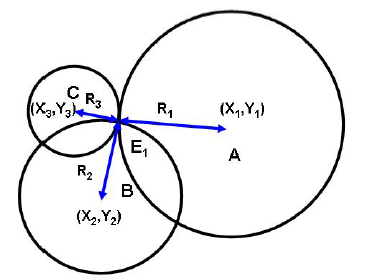
\includegraphics[scale=1]{graphics/triangulation.png}
		\caption{Triangulation\cite{Triangualtion}}
		\label{fig:triangulation}
	\end{center}
\end{figure}

%Fingerprinting
Another WI-FI based method to determine indoor positioning is fingerprinting. Fingerprinting is based on signal strength as well as triangulation. It works by calibrating the system such that the signal strength for each point of interest, e.g. each room, is know to the system, thereby when the signal strength form a device is received it can then be compared to the known strength for all rooms and thereby determine what point of interest the device is closest to. This means that a system using fingerprinting can not determine the exact position of a device, but rather which area the device is currently at \cite{fingerprint1}.
 %http://www.cisco.com/c/en/us/td/docs/solutions/Enterprise/Mobility/WiFiLBS-DG/wifich2.html under RSS har vi en formel til at beregne afstand baseret på signalstyrke

%Paragraph?
%What does google do?
There are ways to overcome the GPS issue, Google presents one possible solution. They have made indoor navigation and tracking possible in indoor spaces trough their Indoor Maps project \cite{IPSoverGPS} which lets users map a building by uploading a floor plan of said building. After the floor plan have been accepted, the system will request information about the location of the WI-FI access points in the building. By doing so the system is able to triangulate using the access points as static reference points and combine that information with the GPS location, thereby utilising both technologies to get a more precise position of the device than by using GPS only.

%About Cisco
Cisco has developed a location-aware wireless network system, the Cisco Unified Wireless Network(UWN), which utilises WI-FI triangulation\cite{CiscoTri} and other wireless communication protocols in order to develop indoor location based services\cite{uwn}.
Cisco utilizes the Cisco Mobility Services Engine (MSE) for their system. The MSE makes it possible for Cisco to track the location of up to 25000 network devices at once. It is the MSE that does the calculations to position devices using the data it receives from the access-points\cite{ciscoMSE}.
The building is modelled by the use of an outline of the floor plan. The image will be converted to a coordinate system that is placed on top of the model which is then supplied with the positions of the access points that are set up in the building. From there it is possible to get the relative position of any nearby devices in relation to the origin of a coordinate system. It is these positions that will be used in order to track and analyse wireless devices.

\subsection{RFID Indoor Positioning}
Another solution is to utilise RFID to create checkpoints throughout a building. These checkpoint are placed in doors or other room entrances and thereby utilise a RFID scanner that reports any observed devices which is equipped with a RFID tag\cite{indoor_bin}. 
RFID works by a scanner reading an id form the passing device then sending the tag of the scanned device, the scanners own id and the time-stamp for the scan to a host computer system. By knowing where the scanners are the system can keep track of the devices\cite{RFIDjournal}.

RFID requires auxiliary hardware to set up the checkpoints, and is in addition to this limited to only work at these checkpoints. By analysing the collected data on the host system it is possible to track a device. Thereby it can be know if a device have entered or exited the room. It can however not be know where in the room it is, which makes it difficult to track someone in a large room.
The technology are being used by air Canada, the largest airline in Canada, to track foot carts, and by doing so saving millions of dollars each year\cite{RFIDjournal}.

%Maby should be moved a bit
%This approach has two limitations. The first lies in the need of auxiliary hardware, as the environment in which the system is to operate are not necessarily equipped with the scanners, which will have to be installed. The second downside is the limitations of the system. It is only possible to get new data about a device's position when it has been observed by a scanner, which means there will be much downtime if the device is moving down a hallway or is stationary in a room. It is therefore not possible to get a precise position of a device after it has moved away from a scanner due to the direction in which the device moved in is unknown. A solution to this problem could be to use more scanners or combine the system with more technologies to improve precision and refresh rate.



\subsection{Choice of technology}\label{subsec:cisco}
Due to RFID not being able to position devices at any time, but is rather able to indicate where a device was last registered, it is not optimal for the applications currently being designed. It have therefore been chosen to use a WI-FI based system.
At the university we have access to a sever that runs the Cisco UWN (MSE) software which is set up to monitor every building on campus at Aalborg University. We have chosen to use the data that is available from here as it is comprehensible to set the system up in a new environment. An overview of Cisco can be seen in \cref{fig:cisco_overveiw}. It shows a snippet of a map on which there are positioned some devices identified by their mac-address.

%How do we solve the previous stated problems